%-----------------------------------LICENSE------------------------------------%
%   This file is part of tikz_figures.                                         %
%                                                                              %
%   tikz_figures is free software: you can redistribute it and/or              %
%   modify it it under the terms of the GNU General Public License as          %
%   published by the Free Software Foundation, either version 3 of the         %
%   License, or (at your option) any later version.                            %
%                                                                              %
%   tikz_figures is distributed in the hope that it will be useful,            %
%   but WITHOUT ANY WARRANTY; without even the implied warranty of             %
%   MERCHANTABILITY or FITNESS FOR A PARTICULAR PURPOSE.  See the              %
%   GNU General Public License for more details.                               %
%                                                                              %
%   You should have received a copy of the GNU General Public License along    %
%   with tikz_figures.  If not, see <https://www.gnu.org/licenses/>.           %
%------------------------------------------------------------------------------%

% Use the standalone class for displaying the tikz image on a small PDF.
\documentclass[crop, tikz]{standalone}

% Import the tikz package to use for the drawing.
\usepackage{tikz}

% Load the arrows.meta library.
\usetikzlibrary{arrows.meta}

% Begin the document.
\begin{document}

    % Draw the picture.
    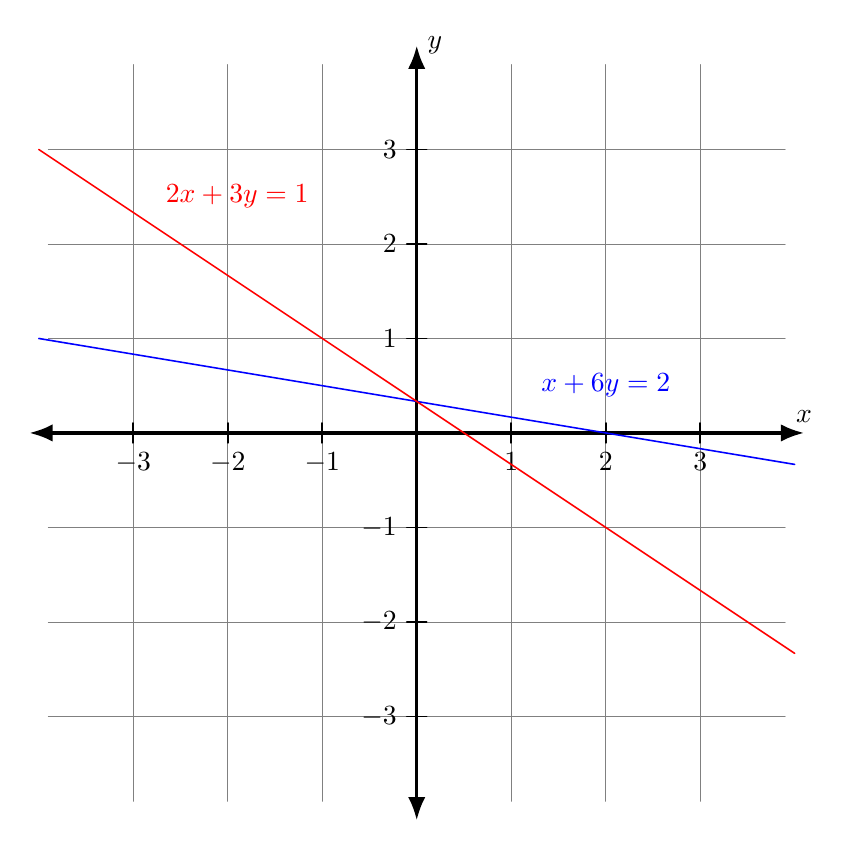
\begin{tikzpicture}[%
        > = Latex,
        line width = 0.2mm,
        line cap = round,
        scale = 1.2
    ]

        % Draw a grid.
        \draw[style = help lines] (-3.9, -3.9) grid (3.9, 3.9);

        % Axes.
        \begin{scope}[very thick]
            \draw[<->] (-4.1, 0.0) to (4.1, 0.0) node [above] {$x$};
            \draw[<->] (0.0, -4.1) to (0.0, 4.1) node [right] {$y$};
        \end{scope}

        % Axes labels.
        \foreach\n in{1, 2, 3}{%
            \draw (\n, 3pt) to (\n, -3pt) node [below] {$\n$};
            \draw (-\n, 3pt) to (-\n, -3pt) node [below] {$-\n$};
            \draw (3pt, \n) to (-3pt, \n) node [left] {$\n$};
            \draw (3pt, -\n) to (-3pt, -\n) node [left] {$-\n$};
        }

        % Draw the lines.
        \draw[draw = blue] (-4.0, 1.0) to (4.0, -0.333);
        \draw[draw = red] (-4.0, 3.0) to (4.0, -2.333);
        \node at (-1.9, 2.5) {$\color{red}2x+3y=1$};
        \node at (2.0, 0.5) {$\color{blue}x+6y=2$};
    \end{tikzpicture}
\end{document}
